%% This is file `thws-mai-pm-template.tex'
%% Created: Magda Gregorova, 30/12/2023
%% Updated: Magda Gregorova, 06/01/2026
%%
%% This is a template for the final papers of the Project Module in the MAI program of the THWS.
%% The template is a minor modification of the SCORES conference template (https://www.scores.si/).
%% I hereby thank the original authors Klemen Berkovi\v{c}, Iztok Fister Jr., Iztok Fister and Luka F\"{u}rst
%% Any errors or problems in this template are my own doing. 
%% The template uses the acmart package https://ctan.org/pkg/acmart?lang=en

%% The first command in your LaTeX source must be the \documentclass command.
%% We use the review anonymous format for submissions - do not change this!
\documentclass[sigconf, review, nonacm, anonymous]{acmart}
% \documentclass[sigconf, nonacm]{acmart}

%% \BibTeX command to typeset BibTeX logo in the docs
\AtBeginDocument{\providecommand\BibTeX{{Bib\TeX}}}

%% Hack to allow for comments about author contribution - not used
% \newcommand{\projectcontrib}[1]{\affiliation{\country{#1}}}

%% If you need any other LaTeX packages, add them here
\usepackage{verbatim}
\usepackage{todonotes}
\usepackage[linesnumbered, boxed, resetcount]{algorithm2e}

%% For managing citations, it is recommended to use bibliography files in BibTeX format.
%%
%% You can then either use BibTeX with the ACM-Reference-Format style, or BibLaTeX with the acmnumeric or acmauthoryear sytles, that include support for advanced citation of software artefact from thebiblatex-software package, also separately available on CTAN.

%% print page numbers
\settopmatter{printfolios=true} 

%% end of the preamble, start of the body of the document source.
\begin{document}

%% The "title" command has an optional parameter allowing the author to define a "short title" to be used in page headers.
\title[A Deep Learning Approach to 3D Human Walking Pose Estimation From SensFloor Capacitive Signals]{A Deep Learning Approach to 3D Human Walking Pose Estimation From SensFloor Capacitive Signals}

%% The "author" command is used to define the authors.
%% You shall submit the anonymised version of your paper for review, so no need to include author names here.
% \author{First Awsomeauthor}
% \affiliation{\institution{THWS, MAI}\city{}\country{}}

% \author{Second Greatauthor}
% \affiliation{\institution{THWS, MAI}\city{}\country{}}

% \author{Third Amazingauthor}
% \affiliation{\institution{THWS, MAI}\city{}\country{}}

% %% By default, the full list of authors will be used in the page headers. 
% %% If this is too long use "shortauthors" to define a more concise list with surnames only.
% \renewcommand{\shortauthors}{Awsomeauthor, Greatauthor, Amazingauthor}

%% The abstract is a short summary of the work to be presented in the article.
\begin{abstract}
While camera-based systems are the dominant approach for human pose estimation, they face challenges in terms of privacy concerns and occlusion problems. These issues are of particular relevance in domains such as elderly care, where pose estimates can be used to monitor residents health or analyze incidents retrospectively. To assess an alternative to camera-based pose estimation, this paper aims to predict 3D walking poses using SensFloor: a capacitance-based floor which registers movement activity. We analyze the potential to utilize the floor's low-resolution signals to estimate poses and to what extent certain joint positions can be predicted accurately. For this purpose, we collected synchronized SensFloor signals and video data, from which we extracted 3D human poses using MediaPipe to serve as ground-truth targets for training. These signals and their corresponding targets were then used for supervised training of an LSTM neural network. To estimate the person's position on the floor, a Kalman filter was applied to smooth the noisy SensFloor measurements. Our results demonstrate that it is possible to predict human walking poses using the proposed methods, establishing a proof-of-concept for an alternative way of activity monitoring.
\end{abstract}

%% Keywords: pick words that accurately describe the work being presented. Separate the keywords with commas - not used.
\keywords{SensFloor, Human pose estimation, Deep Learning, LSTM, Kalman Filter, Capacitive Floor, MediaPipe}
%% This command processes the author and affiliation and title information and builds the first part of the formatted document.
\maketitle

%% Add here the link to your code repository
\vspace{-0.5em}
\textbf{Code:} \url{https://github.com/sensfloor}
\todo{Create README for public organization view}

% Main content
\section{Introduction}
\label{sec:introduction}
% Why are we doing this?

% Introduce sensfloor
% - What type of activities does it detect?
% - What are fields and patches

% Prior research

% Research questions

% Structure/Overview of the paper
% General overview of how to solve the problem (localization and pose prediction)

% Data collection (important: mention how our data looks like)
% - Who did we collect?
% - How does the recording setup look like?
% - Collect video and sensfloor at the same time -> Output: mp4 and csv
% - Creating labels for training using Mediapipe -> Output: Ground truth joint positions in coordinate system with hip as origin

% Describe training of the model
% - Model architecture: Supervised regression model
% - Data split
% - Loss (link loss, MSE)
% - Metrics (PCK, MJPE)
% - Training setup (config) and how we determined the hyperparameters -> Mention what joints we predict here (or in data collection)
% - What is the output?

% Describe localization
% - Sensor & clustering of signals
% - Kalman filter approach
% - Component values
% - What is the output?

% Describe how localization and pose prediction are combined -> Summary that connects training and localization outputs

% How to visualize floor and predicted pose
% - Setup for live predictions
\section{Results}
\label{sec:results}
This section presents an evaluation of the results and a discussion of the model's performance, followed by an examination of the resulting trajectories from the localization pipeline. 

\subsection{SensFloor Pose Estimation Model}
The model training stopped early after 22 epochs with an overall performance of 5.5~cm MPJPE, 87\% PCK@10 and 63\% PCK@5. In the following, we visually compare an estimated to its target pose and analyze the performance across specific joints.

% TEST_MJPE_MEAN: 0.0547 | TEST_MJPE_NOSE: 0.0563 | TEST_MJPE_LEFT_SHOULDER: 0.0410 | TEST_MJPE_RIGHT_SHOULDER: 0.0421 | TEST_MJPE_LEFT_ELBOW: 0.0535 | TEST_MJPE_RIGHT_ELBOW: 0.0548 | TEST_MJPE_LEFT_WRIST: 0.0701 | TEST_MJPE_RIGHT_WRIST: 0.0731 | TEST_MJPE_LEFT_HIP: 0.0205 | TEST_MJPE_RIGHT_HIP: 0.0204 | TEST_MJPE_LEFT_KNEE: 0.0536 | TEST_MJPE_RIGHT_KNEE: 0.0486 | TEST_MJPE_LEFT_ANKLE: 0.0905 | TEST_MJPE_RIGHT_ANKLE: 0.0871
%TEST_PCK_10_MEAN: 0.8674 | TEST_PCK_10_NOSE: 0.8777 | TEST_PCK_10_LEFT_SHOULDER: 0.9364 | TEST_PCK_10_RIGHT_SHOULDER: 0.9350 | TEST_PCK_10_LEFT_ELBOW: 0.8815 | TEST_PCK_10_RIGHT_ELBOW: 0.8826 | TEST_PCK_10_LEFT_WRIST: 0.8102 | TEST_PCK_10_RIGHT_WRIST: 0.7880 | TEST_PCK_10_LEFT_HIP: 0.9858 | TEST_PCK_10_RIGHT_HIP: 0.9856 | TEST_PCK_10_LEFT_KNEE: 0.8714 | TEST_PCK_10_RIGHT_KNEE: 0.8989 | TEST_PCK_10_LEFT_ANKLE: 0.7045 | TEST_PCK_10_RIGHT_ANKLE: 0.7183
%TEST_PCK_5_MEAN: 0.6291 | TEST_PCK_5_NOSE: 0.5960 | TEST_PCK_5_LEFT_SHOULDER: 0.7459 | TEST_PCK_5_RIGHT_SHOULDER: 0.7492 | TEST_PCK_5_LEFT_ELBOW: 0.6339 | TEST_PCK_5_RIGHT_ELBOW: 0.6144 | TEST_PCK_5_LEFT_WRIST: 0.4841 | TEST_PCK_5_RIGHT_WRIST: 0.4634 | TEST_PCK_5_LEFT_HIP: 0.9265 | TEST_PCK_5_RIGHT_HIP: 0.9272 | TEST_PCK_5_LEFT_KNEE: 0.6352 | TEST_PCK_5_RIGHT_KNEE: 0.6728 | TEST_PCK_5_LEFT_ANKLE: 0.3553 | TEST_PCK_5_RIGHT_ANKLE: 0.3739

\subsubsection{Visual Comparison of Estimated and Target Pose} Figure \ref{fig:pose-comparison} illustrates a visual comparison between the estimated pose and the corresponding ground-truth from the test set, shown from four perspectives rotated at 0°, 90°, 180° and 270° angles. Overall, the estimated pose captures the global body posture of the target well. In particular, the global orientation of the skeleton and the left-leg joint positions align closely with the ground-truth. However, discrepancies are visible in the right lower leg, which appears shifted further back relative to the ground-truth. Furthermore, the estimated upper body exhibits a slightly stronger forward lean than the reference.

\begin{figure}[htbp] 
    \centering
    \includegraphics[width=\columnwidth]{img/pose_comparison.pdf}
    \caption{Comparison of a single estimated 3D pose (red) to its corresponding ground-truth pose (black) from four different perspectives.}
    \Description{}
    \label{fig:pose-comparison}
\end{figure}

\subsubsection{Joint Estimations}
Our recorded metrics for the test set, illustrated in Figure \ref{fig:mpjpe}, mirror the results of the visual comparison. The hip was the easiest joint to estimate with about 2~cm median error, because in the poses' local coordinate system, they mostly rotate proximal around the origin and do not move a lot.
In contrast, the wrists and ankles as the most distal joints, move the most and performed the worst, with a median of approximately 5~cm and 7~cm and a bigger interquartile range (IQR). If the model always predicted the mean pose, the overall error of all test-targets would be around 22~cm for wrists and 18~cm for the ankles. Compared to this baseline, this is a significant improvement.  

\begin{figure}[htbp]
    \centering
    \includegraphics[width=\columnwidth]{img/mpjpe_boxplot.pdf}
    \caption{Boxplot of Mean Per Joint Position Error (MPJPE) for each joint on test set with $n=21898$ samples. The box indicates the interquartile range and the whiskers mark the $5^{th}$ and $95^{th}$ percentile.} %TODO: remove samples if not enough space
    \Description{}
    \label{fig:mpjpe}
\end{figure}

Though, while most of the data has a reasonable error, there is a significant portion with higher errors. We explained this for two reasons: First, when the subject performs an unforeseen action by rapidly changing the directions or moving their body unnaturally for example by looking at their watch, the model is not able to predict this.
Second, when the subject has just entered the SensFloor, there is no history information available and the model guesses the stepping foot. Empirical tests during inference confirmed these sources of error.

Furthermore, the ankles exhibit a significantly higher error than the elbows and wrists. This finding is counterintuitive, as the proximity of the ankles to the floor would suggest a higher localization accuracy for these joints. A potential explanation for this may lie in the target pose extraction. MediaPipe tends to estimate the same bone lengths across subjects of varying heights. These fixed proportions may lead to a misalignment between the SensFloor signals and the corresponding joint coordinates, which most significantly impacts the joints close to the floor.


\subsection{Localization and Kalman-Filter Effect}
In \ref{subsec:localization}, we introduced our approach for extracting information about the person's current global position from the SensFloor activation signals. The left side of Figure \ref{fig:kalman-filter-effect} shows the raw clustering position trajectory we recorded during a test walk. The illustrated trajectory is highly erratic. This instability is caused by two main factors. First, the algorithm creates jumps in the estimated position as the mean shifts abruptly whenever a foot makes or breaks contact with the floor. Second, the SensFloor fields produce significant background noise, even in areas where no activity takes place. While increasing the noise signal threshold suppresses some of the noise, it is not a universal solution, as signal intensity of people moving on the floor varies depending on the person's footwear. 

However, applying the Kalman filter largely reduces these issues, as illustrated on the right side of Figure \ref{fig:kalman-filter-effect}. By smoothing out the abrupt transitions and mitigating the impact of outliers, the filter produces a smooth and, according to our empirical evaluation, accurate trajectory.

\begin{figure}[htbp]
    \centering
    \includegraphics[width=\columnwidth]{img/kalman-filter-effect.pdf}
    \caption{Comparison of raw (left) and filtered (right) localization trajectories. The arrows indicate the direction of the movement, a smaller movement results in a smaller arrow.}
    \Description{}
    \label{fig:kalman-filter-effect}
\end{figure}
% - Inference works



% - evaluation
    % - Mediapipe inconsistency
    % - Only male subjects for training
    % - No groundtruth for kalman filter
    % - test set split? No evaluation that our test and trianing set have a similar distribution
    % - Model learned to Look down
    % - Only small sequences of walking possible due to the small floor (and missing API endpoint)
    % - Very limited training set with 
\section{Discussion and Conclusion}
\label{sec:discussion-and-conclusion}

%% The next two lines define the bibliography style to be used, and
%% the bibliography file.
\bibliographystyle{ACM-Reference-Format}
\bibliography{references}

%% We use anonymised submissions for review, so do not include acknowledgements here.
% \section*{Acknowledgements}
% We thank Prof. Dr. Expert Inthefield for supervising our project and PhDStudent VeryHelpful for his valuable advice on many things we would otherwise never figure out.

%% If your work needs an appendix, this is the place to put it.
%\appendix

\end{document}
%% End of file `thws-mai-pm-template.tex'



